\section{Рабочий проект}

Рабочий проект отражает стадию реализации компонентно-ориентированной
программной системы. В данном разделе приводится спецификация реализованных
классов, описание демонстрационных сцен, тестовые наборы для модульного и
регрессионного тестирования, а также результаты системного тестирования
программной основы для построения интерактивных приложений на языке Java.

В рабочем проекте рассматриваются программные компоненты, из которых состоит
разработанная система: ядро ECS, классы управления приложением и сценами,
компоненты объектов, графические и ресурсные классы, системы обработки,
физическая подсистема и демонстрационные сцены.

\subsection{Спецификация компонентов программной системы}

Исходный код программной системы разделен на пакеты по функциональному
назначению. Такое разделение соответствует практикам организации Java-кода и
проектирования программных интерфейсов \cite{bloch-effective-java,horstmann-java-core},
а также позволяет отдельно развивать ядро компонентной модели, прикладные
компоненты сцены, графическую подсистему, физическую подсистему, средства ввода
и демонстрационные примеры.

Основные группы классов программной системы приведены в таблице~\ref{tab:component-groups}.

\begingroup
\small
\renewcommand{\arraystretch}{1.15}
\begin{xltabular}{\textwidth}{|p{0.25\textwidth}|p{0.28\textwidth}|X|}
\caption{Группы классов программной системы\label{tab:component-groups}}\\
\hline
\centrow Группа классов & \centrow Пакеты & \centrow Назначение \\
\hline
\endfirsthead
\caption*{Продолжение таблицы \ref{tab:component-groups}}\\
\hline
\centrow Группа классов & \centrow Пакеты & \centrow Назначение \\
\hline
\finishhead
Ядро компонентной модели & \texttt{qchromatic.jecse.core} & Реализует сущности, компоненты, системы обработки, запросы сущностей и общий жизненный цикл объектов ECS. \\
\hline
Управление приложением и сценами & \texttt{qchromatic.jecse.engine} & Обеспечивает создание приложения, хранение контекста выполнения, загрузку сцен, учет времени, ввод и управление ресурсами. \\
\hline
Компоненты сцены & \texttt{qchromatic.jecse.component} & Описывает прикладные свойства сущностей: трансформацию, камеру, визуальное представление, свет, скрипты, физические тела и коллайдеры. \\
\hline
Графическая подсистема & \texttt{qchromatic.jecse.graphics}, \texttt{qchromatic.jecse.system} & Создает окно, OpenGL-контекст, шейдеры, текстуры, GPU-ресурсы мешей, а также выполняет отрисовку сцены и отладочной геометрии. \\
\hline
Физическая подсистема & \texttt{qchromatic.jecse.component}, \texttt{qchromatic.jecse.system} & Реализует физические тела, коробочные коллайдеры, обнаружение столкновений и импульсное разрешение контактов. \\
\hline
Демонстрационные сцены & \texttt{common.showcase} & Содержит Java-классы, показывающие применение программной системы в 3D-сцене, 2D-интерактивной сцене, текстурированной сцене с освещением и физической сцене. \\
\hline
\end{xltabular}
\renewcommand{\arraystretch}{1.0}
\endgroup

\subsubsection{Вспомогательные математические классы}

Вспомогательные математические классы используются в большинстве подсистем
программной системы и реализуют базовые операции, необходимые для работы с
координатами, поворотами и матрицами преобразований \cite{lengyel-math,dunn-parberry-math}. Через них задаются координаты объектов, направления,
цвета, повороты, матрицы модели, вида и проекции. Эти классы не относятся к
отдельной демонстрационной сцене, а образуют общий прикладной слой для
трансформаций, рендеринга, камеры, ввода и физической подсистемы.

Спецификация вспомогательных математических классов приведена в
таблице~\ref{tab:math-classes}.

\begingroup
\small
\renewcommand{\arraystretch}{1.12}
\begin{xltabular}{\textwidth}{|p{0.22\textwidth}|p{0.30\textwidth}|X|}
\caption{Спецификация вспомогательных математических классов\label{tab:math-classes}}\\
\hline
\centrow Класс & \centrow Основные поля и методы & \centrow Назначение \\
\hline
\endfirsthead
\caption*{Продолжение таблицы \ref{tab:math-classes}}\\
\hline
\centrow Класс & \centrow Основные поля и методы & \centrow Назначение \\
\hline
\finishhead
\texttt{Vec2} & \texttt{x}, \texttt{y}, \texttt{add}, \texttt{mul}, \texttt{length}, \texttt{normalized}, \texttt{dot} & Описывает двумерные величины. Используется для координат мыши, смещения курсора, прокрутки и расчетов в двумерных демонстрационных сценах. \\
\hline
\texttt{Vec3} & \texttt{x}, \texttt{y}, \texttt{z}, \texttt{add}, \texttt{mul}, \texttt{length}, \texttt{normalized}, \texttt{cross}, \texttt{dot} & Описывает трехмерные векторы. Применяется для положения, масштаба, направления движения, скорости, сил, нормалей столкновений и направления источника света. \\
\hline
\texttt{Vec4} & \texttt{x}, \texttt{y}, \texttt{z}, \texttt{w}, \texttt{add}, \texttt{mul}, \texttt{length}, \texttt{normalized}, \texttt{dot} & Хранит четырехкомпонентные значения. Используется для цветов материалов и света, а также для передачи uniform-параметров в графическую подсистему. \\
\hline
\texttt{Mat4} & \texttt{identity}, \texttt{mul}, \texttt{transformPoint}, \texttt{translation}, \texttt{rotation}, \texttt{scale}, \texttt{frustum}, \texttt{ortho} & Реализует матрицу 4x4. Используется для построения матриц модели, вида и проекции, а также для преобразования точек между пространствами сцены. \\
\hline
\texttt{Quaternion} & \texttt{identity}, \texttt{axisAngle}, \texttt{euler}, \texttt{mul}, \texttt{normalize}, \texttt{rotate}, \texttt{forward}, \texttt{right}, \texttt{up}, \texttt{toMat4} & Описывает поворот объекта без накопления лишних угловых ошибок, формирует направления камеры и объектов, а также преобразуется в матрицу поворота. \\
\hline
\end{xltabular}
\renewcommand{\arraystretch}{1.0}
\endgroup

\subsubsection{Классы ядра компонентной модели}

Ядро компонентной модели реализует базовые элементы ECS-архитектуры. Сущность
не содержит прикладной логики сама по себе, а получает поведение через набор
компонентов и обработку системами. Компоненты хранят состояние объекта, системы
выполняют обработку сущностей сцены, а запросы сущностей позволяют получать
только те объекты, которые имеют необходимый набор компонентов.

Спецификация основных классов ядра компонентной модели приведена в
таблице~\ref{tab:ecs-classes}.

\begingroup
\small
\renewcommand{\arraystretch}{1.12}
\begin{xltabular}{\textwidth}{|p{0.22\textwidth}|p{0.26\textwidth}|X|}
\caption{Спецификация классов ядра компонентной модели\label{tab:ecs-classes}}\\
\hline
\centrow Класс & \centrow Основные поля и методы & \centrow Назначение \\
\hline
\endfirsthead
\caption*{Продолжение таблицы \ref{tab:ecs-classes}}\\
\hline
\centrow Класс & \centrow Основные поля и методы & \centrow Назначение \\
\hline
\finishhead
\texttt{Entity} & \texttt{id}, \texttt{addComponent}, \texttt{getComponent}, \texttt{removeComponent}, \texttt{hasComponent}, \texttt{components} & Хранит уникальный идентификатор сущности и набор компонентов. Обеспечивает добавление, получение и удаление компонентов. При изменении состава компонентов уведомляет наблюдателя сцены. \\
\hline
\texttt{Component} & \texttt{entity}, \texttt{started}, \texttt{destroyed}, \texttt{onAttach}, \texttt{onStart}, \texttt{onStop}, \texttt{onDestroy} & Является базовым классом для всех компонентов. Хранит ссылку на сущность и управляет жизненным циклом компонента: присоединение, запуск, остановка, уничтожение. \\
\hline
\texttt{System} & \texttt{init}, \texttt{start}, \texttt{loop}, \texttt{stop}, \texttt{destroy}, \texttt{order}, \texttt{scene} & Является базовым классом для систем обработки. Позволяет выполнять код на разных стадиях жизненного цикла сцены и задавать порядок выполнения систем. \\
\hline
\texttt{EntityQuery} & \texttt{matches}, \texttt{update}, \texttt{contains}, \texttt{snapshot}, \texttt{iterator} & Хранит выборку сущностей, соответствующих набору обязательных компонентов. Используется системами для обхода только подходящих объектов сцены. \\
\hline
\texttt{EntityObserver} & \texttt{onComponentAdded}, \texttt{onComponentRemoved} & Определяет интерфейс уведомлений о добавлении и удалении компонентов. В реализации сцены используется для обновления индексов и запросов сущностей. \\
\hline
\texttt{Disposable} & \texttt{destroy} & Определяет единый интерфейс освобождения ресурсов. Используется для компонентов и графических объектов, которые требуют явного уничтожения. \\
\hline
\end{xltabular}
\renewcommand{\arraystretch}{1.0}
\endgroup

Класс \texttt{Entity} хранит компоненты в отображении по точному классу
компонента. Благодаря этому получение компонента по типу выполняется напрямую,
а сама сущность не может иметь два компонента одного и того же конкретного
класса. Для компонентов-наследников предусмотрены методы, учитывающие
иерархию классов, например \texttt{getComponentsInheritance} и
\texttt{hasComponentInheritance}. Это используется в скриптовой подсистеме,
где пользовательские скрипты являются наследниками базового класса
\texttt{Script}.

\subsubsection{Классы управления приложением и сценами}

Классы управления приложением связывают ECS-ядро с окном, пользовательским
вводом, ресурсами и временем. Основной цикл приложения находится в классе
\texttt{Application}. Сцена хранит сущности и системы обработки, а менеджер
сцен отвечает за загрузку, замену и уничтожение активной сцены.

Спецификация основных классов управления приложением приведена в
таблице~\ref{tab:engine-classes}.

\begingroup
\small
\renewcommand{\arraystretch}{1.12}
\begin{xltabular}{\textwidth}{|p{0.22\textwidth}|p{0.26\textwidth}|X|}
\caption{Спецификация классов управления приложением и сценами\label{tab:engine-classes}}\\
\hline
\centrow Класс & \centrow Основные поля и методы & \centrow Назначение \\
\hline
\endfirsthead
\caption*{Продолжение таблицы \ref{tab:engine-classes}}\\
\hline
\centrow Класс & \centrow Основные поля и методы & \centrow Назначение \\
\hline
\finishhead
\texttt{Application} & \texttt{run}, \texttt{context}, \texttt{getWindow} & Создает контекст программной системы, запускает основной цикл, обновляет время, активную сцену, ввод, окно и освобождает ресурсы после завершения работы. \\
\hline
\texttt{EngineConfig} & \texttt{clearColor}, \texttt{fixedDeltaTime}, \texttt{timeScale}, \texttt{autoUpdateCameraAspect}, \texttt{debugOpenGLErrors} & Хранит параметры запуска программной системы: цвет очистки экрана, фиксированный шаг времени, масштаб времени, автоматическое обновление соотношения сторон камеры и режим проверки ошибок OpenGL. \\
\hline
\texttt{EngineContext} & \texttt{use}, \texttt{current}, \texttt{input}, \texttt{assets}, \texttt{sceneManager}, \texttt{time}, \texttt{window}, \texttt{destroy} & Хранит текущие экземпляры подсистем приложения и делает их доступными из статических фасадов. Освобождает активную сцену, ресурсы и окно при завершении приложения. \\
\hline
\texttt{Scene} & \texttt{init}, \texttt{start}, \texttt{loop}, \texttt{stop}, \texttt{dispose}, \texttt{addEntity}, \texttt{removeEntity}, \texttt{addSystem}, \texttt{query} & Хранит сущности, системы, индексы компонентов и запросы сущностей. Управляет жизненным циклом компонентов и систем, а также выполняет отложенные структурные изменения. \\
\hline
\texttt{SceneManager} & \texttt{load}, \texttt{replace}, \texttt{requestLoad}, \texttt{requestReplace}, \texttt{applyPendingChanges}, \texttt{disposeActiveScene} & Управляет активной сценой. Поддерживает немедленную загрузку и замену сцены, а также отложенную замену, безопасную для вызова из пользовательских скриптов. \\
\hline
\texttt{Time} & \texttt{reset}, \texttt{update}, \texttt{deltaTime}, \texttt{unscaledDeltaTime}, \texttt{time}, \texttt{frame} & Хранит время приложения, длительность текущего кадра, не масштабированное время, номер кадра и параметры масштаба времени. \\
\hline
\texttt{InputState} & \texttt{setKeyState}, \texttt{setMousePosition}, \texttt{setScrollOffset}, \texttt{getKey}, \texttt{getKeyDown}, \texttt{getMouseDelta}, \texttt{update} & Хранит состояние клавиатуры, мыши, прокрутки и смещение курсора между кадрами. Позволяет отличать удержание клавиши от однократного нажатия. \\
\hline
\texttt{Input} & \texttt{use}, \texttt{getKey}, \texttt{getKeyDown}, \texttt{getMousePosition}, \texttt{getMouseDelta}, \texttt{getMouseScroll} & Статический фасад для доступа к текущему состоянию ввода из пользовательских скриптов и систем. \\
\hline
\texttt{KeyCode} & \texttt{A--Z}, \texttt{ALPHA\_0--ALPHA\_9}, \texttt{F1--F12}, \texttt{UP}, \texttt{DOWN}, \texttt{LEFT}, \texttt{RIGHT}, \texttt{MB\_1--MB\_8} & Предоставляет именованные константы клавиатуры и мыши, связанные с кодами GLFW. Используется в пользовательских скриптах для читаемой обработки ввода. \\
\hline
\end{xltabular}
\renewcommand{\arraystretch}{1.0}
\endgroup

Особое значение имеет механизм отложенных структурных изменений в классе
\texttt{Scene}. Если сущность, компонент или система добавляются либо удаляются
во время обхода систем, действие помещается в очередь и выполняется после
завершения небезопасного участка обновления. Такой подход предотвращает ошибки,
связанные с изменением коллекций во время их обхода, и позволяет вызывать
изменения структуры сцены из пользовательских скриптов.

\subsubsection{Компоненты сцены}

Компоненты сцены описывают данные, которые могут быть добавлены к сущностям.
Именно набор компонентов определяет, будет ли сущность отображаться, участвовать
в физике, выполнять пользовательский скрипт или использоваться как камера.

Спецификация основных компонентов сцены приведена в таблице~\ref{tab:scene-components}.

\begingroup
\small
\renewcommand{\arraystretch}{1.12}
\begin{xltabular}{\textwidth}{|p{0.22\textwidth}|p{0.26\textwidth}|X|}
\caption{Спецификация компонентов сцены\label{tab:scene-components}}\\
\hline
\centrow Компонент & \centrow Основные поля и методы & \centrow Назначение \\
\hline
\endfirsthead
\caption*{Продолжение таблицы \ref{tab:scene-components}}\\
\hline
\centrow Компонент & \centrow Основные поля и методы & \centrow Назначение \\
\hline
\finishhead
\texttt{Transform} & \texttt{position}, \texttt{rotation}, \texttt{scale}, \texttt{parent}, \texttt{children}, \texttt{worldPosition}, \texttt{getModelMatrix} & Хранит положение, поворот, масштаб и иерархию трансформаций. Формирует локальную и мировую матрицы объекта. \\
\hline
\texttt{Camera} & \texttt{ortho}, \texttt{fov}, \texttt{orthoSize}, \texttt{aspectRatio}, \texttt{near}, \texttt{far}, \texttt{priority}, \texttt{cullingMask}, \texttt{getViewMatrix}, \texttt{getProjectionMatrix} & Описывает перспективную или ортографическую камеру. Формирует матрицы вида и проекции, задает приоритет камеры и маску видимости слоев. \\
\hline
\texttt{MeshRenderer} & \texttt{mesh}, \texttt{material}, \texttt{enabled}, \texttt{layer}, \texttt{renderQueue}, \texttt{boundsRadius} & Связывает сущность с геометрией и материалом. Используется системой рендеринга для построения очереди отображения. \\
\hline
\texttt{DirectionalLight} & \texttt{direction}, \texttt{color}, \texttt{intensity}, \texttt{enabled} & Описывает направленный источник света, применяемый при отрисовке материалов с освещением. \\
\hline
\texttt{Script} & \texttt{init}, \texttt{start}, \texttt{loop}, \texttt{stop}, \texttt{destroy} & Базовый класс пользовательского поведения. Подключается к сущности как компонент и обрабатывается \texttt{ScriptSystem}. \\
\hline
\texttt{Rigidbody} & \texttt{type}, \texttt{velocity}, \texttt{angularVelocity}, \texttt{addForce}, \texttt{addImpulse}, \texttt{mass}, \texttt{useGravity}, \texttt{sleep}, \texttt{wakeUp} & Описывает физическое тело. Хранит тип тела, скорость, угловую скорость, массу, силы, импульсы, демпфирование и состояние сна. \\
\hline
\texttt{Collider} & \texttt{enabled}, \texttt{trigger}, \texttt{offset}, \texttt{layer}, \texttt{mask}, \texttt{restitution}, \texttt{friction} & Базовый класс коллайдера. Задает активность, смещение, слой столкновений, маску взаимодействия, упругость и трение. \\
\hline
\texttt{BoxCollider} & \texttt{halfExtents}, \texttt{size} & Реализует коробочный коллайдер. Задает половинные размеры или полный размер параллелепипеда, участвующего в физическом расчете. \\
\hline
\end{xltabular}
\renewcommand{\arraystretch}{1.0}
\endgroup

В компонентах используется цепочечный стиль настройки, при котором метод
изменения параметра возвращает сам объект. Благодаря этому сущность сцены может
создаваться компактно: сначала создается \texttt{Entity}, затем последовательно
добавляются \texttt{Transform}, \texttt{MeshRenderer}, \texttt{Rigidbody},
\texttt{BoxCollider} и другие компоненты.

\subsubsection{Графические и ресурсные классы}

Графическая подсистема реализует создание окна, управление OpenGL-ресурсами,
шейдерами, текстурами и материалами. Часть классов работает напрямую с нативными
ресурсами и поэтому реализует явное освобождение памяти и объектов OpenGL.

Спецификация основных графических и ресурсных классов приведена в
таблице~\ref{tab:rp-graphics-classes}.

\begingroup
\small
\renewcommand{\arraystretch}{1.12}
\begin{xltabular}{\textwidth}{|p{0.22\textwidth}|p{0.26\textwidth}|X|}
\caption{Спецификация графических и ресурсных классов\label{tab:rp-graphics-classes}}\\
\hline
\centrow Класс & \centrow Основные поля и методы & \centrow Назначение \\
\hline
\endfirsthead
\caption*{Продолжение таблицы \ref{tab:rp-graphics-classes}}\\
\hline
\centrow Класс & \centrow Основные поля и методы & \centrow Назначение \\
\hline
\finishhead
\texttt{Window} & \texttt{show}, \texttt{clear}, \texttt{update}, \texttt{destroy}, \texttt{shouldClose}, \texttt{aspectRatio}, \texttt{setCursorDisabled}, \texttt{addResizeListener} & Создает GLFW-окно, OpenGL-контекст, регистрирует обработчики ввода и обновляет состояние окна в основном цикле. \\
\hline
\texttt{Shader} & \texttt{use}, \texttt{setUniform}, \texttt{getUniformLocation}, \texttt{destroy} & Загружает и компилирует GLSL-шейдеры, линкует программу OpenGL, кэширует расположения uniform-переменных и передает значения в шейдер. \\
\hline
\texttt{Texture} & \texttt{load}, \texttt{debugTexture}, \texttt{setPixel}, \texttt{uploadToGPU}, \texttt{bind}, \texttt{destroy} & Загружает текстуры из файлов через STB или создает процедурные изображения, передает данные в OpenGL и освобождает объект текстуры. \\
\hline
\texttt{Mesh} & \texttt{vertices}, \texttt{triangles}, \texttt{vertexStride}, \texttt{vertexCount}, \texttt{indexCount}, \texttt{version} & Хранит массив вершин, индексы треугольников, шаг вершины и номер версии геометрии для обновления GPU-ресурса при изменении меша. \\
\hline
\texttt{Meshes} & \texttt{triangle}, \texttt{quad}, \texttt{cube} & Предоставляет фабричные методы для создания базовой геометрии: треугольника, прямоугольника и куба. \\
\hline
\texttt{Material} & \texttt{use}, \texttt{shader}, \texttt{texture}, \texttt{color}, \texttt{set}, \texttt{setTexture} & Хранит шейдер, набор uniform-параметров и текстуры. Перед отрисовкой активирует шейдер, привязывает текстуры и передает параметры материала. \\
\hline
\texttt{AssetManager} & \texttt{shader}, \texttt{basicShader}, \texttt{debugTexture}, \texttt{texture}, \texttt{destroy} & Кэширует шейдеры и текстуры по строковым ключам, предотвращает повторную загрузку одинаковых ресурсов и освобождает их при завершении приложения. \\
\hline
\texttt{Assets} & \texttt{use}, \texttt{basicShader}, \texttt{debugTexture}, \texttt{texture} & Статический фасад для доступа к текущему менеджеру ресурсов из разных частей программы. \\
\hline
\texttt{MeshGpuResource} & \texttt{vaoId}, \texttt{vboId}, \texttt{eboId}, \texttt{meshVersion}, \texttt{indexCount}, \texttt{destroy} & Хранит идентификаторы VAO, VBO и EBO, связанные с конкретной версией меша, и удаляет соответствующие OpenGL-объекты. \\
\hline
\texttt{DebugRenderer} & \texttt{line}, \texttt{axis}, \texttt{bounds}, \texttt{consumeLines}, \texttt{clear} & Накапливает отладочные линии на кадр. Используется для отображения осей, границ объектов, коллайдеров и вспомогательной сетки. \\
\hline
\texttt{Shaders} & \texttt{basic} & Предоставляет краткий доступ к стандартному шейдеру программной системы через фасад ресурсов. Упрощает создание базовых материалов в демонстрационных сценах. \\
\hline
\texttt{WindowResizeListener} & \texttt{onResize} & Определяет интерфейс обратного вызова при изменении размеров окна. Используется для реакции подсистем на изменение ширины, высоты и соотношения сторон. \\
\hline
\end{xltabular}
\renewcommand{\arraystretch}{1.0}
\endgroup

Для типового использования разработчик не должен напрямую создавать VAO, VBO и
EBO. Эти операции скрыты внутри системы рендеринга и класса
\texttt{MeshGpuResource}. При изменении версии меша старый GPU-ресурс уничтожается
и создается новый.

\subsubsection{Системы обработки}

Системы обработки реализуют поведение сцены на каждом кадре. Каждая система
получает доступ к сцене, формирует запросы сущностей и выполняет обработку
только подходящих объектов. Порядок выполнения задается числовым значением
\texttt{order} базового класса \texttt{System}.

Спецификация систем обработки приведена в таблице~\ref{tab:systems}.

\begingroup
\small
\renewcommand{\arraystretch}{1.12}
\begin{xltabular}{\textwidth}{|p{0.23\textwidth}|p{0.27\textwidth}|X|}
\caption{Спецификация систем обработки\label{tab:systems}}\\
\hline
\centrow Система & \centrow Используемые компоненты & \centrow Выполняемые функции \\
\hline
\endfirsthead
\caption*{Продолжение таблицы \ref{tab:systems}}\\
\hline
\centrow Система & \centrow Используемые компоненты & \centrow Выполняемые функции \\
\hline
\finishhead
\texttt{ScriptSystem} & \texttt{Script} и его наследники & Находит пользовательские скрипты, вызывает методы \texttt{init}, \texttt{start}, \texttt{loop}, \texttt{stop}, \texttt{destroy}, реагирует на добавление и удаление скриптов во время работы сцены. \\
\hline
\texttt{PhysicsSystem} & \texttt{Transform}, \texttt{Rigidbody}, \texttt{Collider}, \texttt{BoxCollider} & Выполняет фиксированный физический шаг, применяет силы и гравитацию, интегрирует скорости и положения, обнаруживает столкновения коробочных коллайдеров, разрешает контакты и отображает коллайдеры в режиме отладки. \\
\hline
\texttt{RenderSystem} & \texttt{Transform}, \texttt{MeshRenderer}, \texttt{Camera}, \texttt{DirectionalLight} & Выбирает активную камеру и источник света, строит очередь команд отрисовки, проверяет слои и видимость, сортирует команды и выполняет вызовы OpenGL для отображения мешей. \\
\hline
\texttt{DebugRenderSystem} & \texttt{Transform}, \texttt{Camera}; данные \texttt{DebugRenderer} & Получает накопленные отладочные линии, формирует динамический буфер вершин и рисует вспомогательную геометрию поверх основной сцены. \\
\hline
\end{xltabular}
\renewcommand{\arraystretch}{1.0}
\endgroup

Для реализации рендеринга и физики используются внутренние служебные структуры.
Они не входят в публичный API, но важны для понимания рабочего проекта, так как
показывают, каким образом системы обработки подготавливают данные кадра и
результаты столкновений. Основные внутренние структуры систем обработки
приведены в таблице~\ref{tab:system-internal-structures}.

\begingroup
\small
\renewcommand{\arraystretch}{1.12}
\begin{xltabular}{\textwidth}{|p{0.24\textwidth}|p{0.24\textwidth}|X|}
\caption{Внутренние структуры систем обработки\label{tab:system-internal-structures}}\\
\hline
\centrow Структура & \centrow Система & \centrow Назначение \\
\hline
\endfirsthead
\caption*{Продолжение таблицы \ref{tab:system-internal-structures}}\\
\hline
\centrow Структура & \centrow Система & \centrow Назначение \\
\hline
\finishhead
\texttt{RenderCommand} & \texttt{RenderSystem} & Хранит меш, материал, трансформацию и номер очереди отрисовки. На основе этих структур формируется упорядоченный список объектов, которые должны быть отображены в текущем кадре. \\
\hline
\texttt{LightState} & \texttt{RenderSystem} & Хранит подготовленные параметры направленного света: направление, цвет и признак активности. Передается в материал перед выполнением команд отрисовки. \\
\hline
\texttt{ColliderEntry} & \texttt{PhysicsSystem} & Связывает сущность, трансформацию, физическое тело, коллайдер и вычисленную физическую форму. Используется при поиске пар объектов для проверки столкновений. \\
\hline
\texttt{BoxShape} & \texttt{PhysicsSystem} & Описывает коробочную форму в мировых координатах: центр, локальные оси, половинные размеры и граничные значения. Нужна для SAT-проверки и отладочной визуализации. \\
\hline
\texttt{SatResult} & \texttt{PhysicsSystem} & Хранит результат проверки пересечения коробок методом разделяющих осей: минимальную глубину проникновения и нормаль столкновения. \\
\hline
\texttt{Contact} & \texttt{PhysicsSystem} & Описывает контакт двух коллайдеров: участвующие объекты, нормаль, глубину проникновения и набор точек контакта. Используется при позиционной коррекции и импульсном разрешении столкновения. \\
\hline
\end{xltabular}
\renewcommand{\arraystretch}{1.0}
\endgroup

В демонстрационных сценах используется следующий типовой порядок выполнения
систем: сначала \texttt{ScriptSystem}, затем \texttt{PhysicsSystem}, затем
\texttt{RenderSystem} и \texttt{DebugRenderSystem}. Благодаря этому пользовательские
скрипты успевают обработать ввод, физическая подсистема обновляет состояние тел,
после чего графическая подсистема отображает уже измененную сцену.

\subsubsection{Демонстрационные сцены}

Демонстрационные сцены реализованы как самостоятельные Java-классы с методом
\texttt{main}. Каждая сцена создает приложение, настраивает окно, формирует объект
\texttt{Scene}, добавляет в него системы обработки, сущности и компоненты, после
чего запускает основной цикл приложения. Сцены не используют визуальный редактор
и показывают, что программная система может применяться через Java API.

Спецификация демонстрационных сцен приведена в таблице~\ref{tab:demo-scene-spec}.

\begingroup
\small
\renewcommand{\arraystretch}{1.12}
\begin{xltabular}{\textwidth}{|p{0.23\textwidth}|p{0.31\textwidth}|X|}
\caption{Спецификация демонстрационных сцен\label{tab:demo-scene-spec}}\\
\hline
\centrow Сцена & \centrow Состав сцены & \centrow Назначение реализации \\
\hline
\endfirsthead
\caption*{Продолжение таблицы \ref{tab:demo-scene-spec}}\\
\hline
\centrow Сцена & \centrow Состав сцены & \centrow Назначение реализации \\
\hline
\finishhead
\texttt{ShowcaseScene} & Перспективная камера, свободное управление камерой, направленный свет, корневой и дочерний кубы, пол, объект на отдельном слое, скрытый объект, отладочные направляющие. & Демонстрирует базовый трехмерный рендеринг, иерархию \texttt{Transform}, работу камеры, слои видимости, отсечение объектов, вращение объектов через скрипты и отладочную геометрию. \\
\hline
\texttt{Interactive2DScene} & Ортографическая камера, фон, интерактивная кнопка изменения цвета, переключатель вращения, пульсирующий объект, слайдер и скрипт отслеживания координат мыши. & Демонстрирует применение той же компонентной архитектуры для двумерной интерактивной сцены с обработкой курсора, кликов мыши и изменением состояния объектов. \\
\hline
\texttt{TexturedLightingScene} & Перспективная камера, свободное управление камерой, анимированный направленный свет, процедурно созданные текстуры травы, земли и камня, набор текстурированных кубов. & Демонстрирует работу материалов, текстур, uniform-параметров, направленного освещения и пользовательского скрипта изменения параметров света во времени. \\
\hline
\texttt{PhysicsScene} & Перспективная камера, свободное управление камерой, направленный свет, пол, узкая опора, движущаяся кинематическая платформа, статические стены, динамические кубы, отладочная сетка и визуализация коллайдеров. & Демонстрирует совместную работу скриптов, физики, рендеринга, ввода, перезапуска сцены и отладочной визуализации физической подсистемы. \\
\hline
\end{xltabular}
\renewcommand{\arraystretch}{1.0}
\endgroup

Наиболее комплексной демонстрационной сценой является \texttt{PhysicsScene}, так
как она одновременно использует большинство реализованных подсистем. Структура
основных объектов данной сцены приведена в таблице~\ref{tab:physics-scene-entities}.

\begingroup
\small
\renewcommand{\arraystretch}{1.12}
\begin{xltabular}{\textwidth}{|p{0.23\textwidth}|p{0.35\textwidth}|X|}
\caption{Основные объекты сцены \texttt{PhysicsScene}\label{tab:physics-scene-entities}}\\
\hline
\centrow Объект сцены & \centrow Компоненты & \centrow Назначение \\
\hline
\endfirsthead
\caption*{Продолжение таблицы \ref{tab:physics-scene-entities}}\\
\hline
\centrow Объект сцены & \centrow Компоненты & \centrow Назначение \\
\hline
\finishhead
\texttt{sun} & \texttt{DirectionalLight} & Источник направленного света, влияющий на освещение видимых объектов. \\
\hline
\texttt{camera} & \texttt{Transform}, \texttt{Camera}, \texttt{FreecamController} & Камера наблюдателя со свободным перемещением и поворотом по клавиатуре и мыши. \\
\hline
\texttt{kinematic-platform} & \texttt{Transform}, \texttt{Rigidbody}, \texttt{BoxCollider}, \texttt{MeshRenderer}, \texttt{PlatformBounceScript} & Движущаяся кинематическая платформа, которая меняет направление движения в заданных границах и взаимодействует с динамическими объектами. \\
\hline
\texttt{physics-grid} & \texttt{PhysicsGridScript} & Скрипт вывода отладочной сетки на плоскости сцены для визуальной оценки положения объектов. \\
\hline
\texttt{scene-controls} & \texttt{PhysicsSceneControlScript} & Скрипт перезапуска сцены по нажатию клавиши \texttt{R} через отложенную замену сцены в \texttt{SceneManager}. \\
\hline
\texttt{floor} & \texttt{Transform}, \texttt{BoxCollider}, \texttt{MeshRenderer} & Статическая опорная поверхность для падения динамических тел. \\
\hline
\texttt{narrow-support} & \texttt{Transform}, \texttt{BoxCollider}, \texttt{MeshRenderer} & Узкая статическая опора, позволяющая проверить падение тел с края и возникновение вращения при смещенном контакте. \\
\hline
Статические стены & \texttt{Transform}, \texttt{BoxCollider}, \texttt{MeshRenderer} & Ограничивают область сцены и используются для проверки столкновений со стенами. \\
\hline
Динамические кубы & \texttt{Transform}, \texttt{Rigidbody}, \texttt{BoxCollider}, \texttt{MeshRenderer} & Физические тела, падающие под действием гравитации и взаимодействующие с полом, опорами, стенами и кинематической платформой. \\
\hline
\end{xltabular}
\renewcommand{\arraystretch}{1.0}
\endgroup

\subsection{Модульное и регрессионное тестирование программной системы}

Тестирование программной системы выполнялось по наборам проверок, для которых
фиксировались входные данные, ожидаемый результат и фактическое поведение. Такой
подход соответствует общим принципам систематического тестирования программ
\cite{myers-testing}.

Тестирование выполнено для подсистем, которые могут быть проверены без создания
графического OpenGL-контекста: ядра компонентной модели, подсистемы ввода,
менеджера сцен и физической подсистемы. Подсистемы, зависящие от окна,
OpenGL-ресурсов и действий пользователя, дополнительно проверяются системным
тестированием демонстрационных сцен.

Автоматизированные тесты реализованы как Java-классы с методом \texttt{main}.
При нарушении ожидаемого результата тест выбрасывает \texttt{AssertionError}. Для
ядра компонентной модели дополнительно приведены функциональные тестовые наборы,
которые фиксируют проверяемые сценарии работы сущностей, компонентов и запросов.
Такой формат позволяет воспроизводимо проверять критичные сценарии работы
подсистем и не требует создания графического окна для проверяемых модулей.

\subsubsection{Тестирование ядра компонентной модели}

Так как основой разработанной программной системы является компонентная модель,
отдельно проверялись сценарии работы сущностей, компонентов, запросов и
жизненного цикла сцены. Данные проверки не требуют графического окна и
показывают, что пользователь может строить интерактивное приложение из
самостоятельных объектов, компонентов и систем обработки. Тестовые наборы ядра
компонентной модели приведены в таблице~\ref{tab:ecs-tests}.

\begingroup
\small
\renewcommand{\arraystretch}{1.12}
\begin{xltabular}{\textwidth}{|p{0.30\textwidth}|p{0.34\textwidth}|X|}
\caption{Тестовые наборы ядра компонентной модели\label{tab:ecs-tests}}\\
\hline
\centrow Описание теста & \centrow Входные данные & \centrow Эталонный результат \\
\hline
\endfirsthead
\caption*{Продолжение таблицы \ref{tab:ecs-tests}}\\
\hline
\centrow Описание теста & \centrow Входные данные & \centrow Эталонный результат \\
\hline
\finishhead
Добавление компонента к сущности & Создается сущность \texttt{Entity}, после чего к ней добавляется компонент \texttt{Transform}. & Сущность содержит добавленный компонент, а компонент получает ссылку на свою сущность. \\
\hline
Получение компонента по типу & После добавления \texttt{Transform} вызывается получение компонента по его классу. & Возвращается тот же экземпляр компонента, который был добавлен к сущности. \\
\hline
Проверка наличия компонента & Для сущности с \texttt{Transform} выполняется проверка наличия \texttt{Transform} и \texttt{MeshRenderer}. & Проверка для \texttt{Transform} возвращает положительный результат, проверка для отсутствующего компонента возвращает отрицательный результат. \\
\hline
Удаление компонента & Из сущности удаляется ранее добавленный компонент \texttt{Transform}. & Компонент больше не возвращается при запросе по типу, а сущность исключается из запросов, которым требуется \texttt{Transform}. \\
\hline
Обновление запроса сущностей & В сцене создается запрос на сущности с компонентами \texttt{Transform} и \texttt{MeshRenderer}; затем к сущности последовательно добавляются эти компоненты. & Сущность попадает в выборку только после появления полного набора компонентов. \\
\hline
Отложенное добавление сущности & Во время выполнения цикла сцены система или скрипт запрашивает добавление новой сущности. & Структура сцены не изменяется во время небезопасного обхода, новая сущность появляется после применения отложенных изменений. \\
\hline
Отложенное удаление сущности & Во время выполнения цикла сцены система или скрипт запрашивает удаление существующей сущности. & Сущность удаляется после завершения текущего обхода, связанные компоненты проходят завершающие этапы жизненного цикла. \\
\hline
Вызов жизненного цикла компонента & К сущности добавляется компонент, затем сцена запускается, обновляется и уничтожается. & Для компонента последовательно вызываются методы присоединения, запуска, остановки и уничтожения в соответствии с состоянием сцены. \\
\hline
\end{xltabular}
\renewcommand{\arraystretch}{1.0}
\endgroup

\subsubsection{Тестирование подсистемы ввода}

Тестирование подсистемы ввода выполняется классом \texttt{InputStateTest}.
Проверяется накопление смещения мыши, сохранение позиции курсора, сброс
покадровых данных и накопление прокрутки. Тестовые наборы приведены в
таблице~\ref{tab:input-tests}.

\begingroup
\small
\renewcommand{\arraystretch}{1.12}
\begin{xltabular}{\textwidth}{|p{0.30\textwidth}|p{0.34\textwidth}|X|}
\caption{Тестовые наборы подсистемы ввода\label{tab:input-tests}}\\
\hline
\centrow Описание теста & \centrow Входные данные & \centrow Эталонный результат \\
\hline
\endfirsthead
\caption*{Продолжение таблицы \ref{tab:input-tests}}\\
\hline
\centrow Описание теста & \centrow Входные данные & \centrow Эталонный результат \\
\hline
\finishhead
Первичная установка позиции курсора & Вызов \texttt{setMousePosition(100, 50)} для нового объекта \texttt{InputState}. & Позиция курсора равна \texttt{(100, 50)}, смещение мыши равно \texttt{(0, 0)}, так как предыдущая позиция еще неизвестна. \\
\hline
Накопление смещения курсора в пределах кадра & Последовательные вызовы \texttt{setMousePosition(110, 45)} и \texttt{setMousePosition(125, 40)}. & Смещение мыши за кадр равно \texttt{(25, -10)}. \\
\hline
Сброс покадрового смещения после обновления & Вызов \texttt{update()} после накопления смещения. & Смещение мыши становится \texttt{(0, 0)}, текущая позиция остается \texttt{(125, 40)}. \\
\hline
Сохранение отслеживания позиции после обновления & После \texttt{update()} выполняется \texttt{setMousePosition(130, 35)}. & Смещение мыши равно \texttt{(5, -5)}, так как предыдущая позиция была сохранена. \\
\hline
Сброс отслеживания позиции при повторном входе курсора & Вызовы \texttt{resetMousePositionTracking()} и \texttt{setMousePosition(400, 300)}. & Смещение мыши равно \texttt{(0, 0)}, новая позиция считается первой после сброса. \\
\hline
Накопление прокрутки мыши & Вызовы \texttt{setScrollOffset(0, 1)} и \texttt{setScrollOffset(0, 2)}. & Значение прокрутки равно \texttt{(0, 3)}. \\
\hline
Сброс прокрутки после обновления & Вызов \texttt{update()} после накопления прокрутки. & Значение прокрутки сбрасывается в \texttt{(0, 0)}. \\
\hline
\end{xltabular}
\renewcommand{\arraystretch}{1.0}
\endgroup

\subsubsection{Тестирование менеджера сцен}

Тестирование менеджера сцен выполняется классом \texttt{SceneManagerTest}. В
тесте используется вспомогательная система \texttt{ProbeSystem}, которая фиксирует
факт запуска и уничтожения сцены. Тестовые наборы приведены в
таблице~\ref{tab:scene-manager-tests}.

\begingroup
\small
\renewcommand{\arraystretch}{1.12}
\begin{xltabular}{\textwidth}{|p{0.30\textwidth}|p{0.34\textwidth}|X|}
\caption{Тестовые наборы менеджера сцен\label{tab:scene-manager-tests}}\\
\hline
\centrow Описание теста & \centrow Входные данные & \centrow Эталонный результат \\
\hline
\endfirsthead
\caption*{Продолжение таблицы \ref{tab:scene-manager-tests}}\\
\hline
\centrow Описание теста & \centrow Входные данные & \centrow Эталонный результат \\
\hline
\finishhead
Загрузка первой сцены & Создаются две сцены. В менеджер загружается первая сцена методом \texttt{load}. & Активной сценой становится первая сцена, ее система переходит в состояние запуска. \\
\hline
Запрос отложенной замены сцены & После загрузки первой сцены вызывается \texttt{requestReplace(second)}. & Активная сцена не меняется до вызова \texttt{applyPendingChanges}. \\
\hline
Применение отложенной замены сцены & После запроса замены вызывается \texttt{applyPendingChanges}. & Активной становится вторая сцена, предыдущая сцена уничтожается, система новой сцены запускается. \\
\hline
Освобождение активной сцены & После проверки вызывается \texttt{disposeActiveScene}. & Активная сцена корректно уничтожается, связанные системы получают вызовы завершения жизненного цикла. \\
\hline
\end{xltabular}
\renewcommand{\arraystretch}{1.0}
\endgroup

\subsubsection{Тестирование физической подсистемы}

Тестирование физической подсистемы выполняется классом \texttt{PhysicsSystemTest}.
Тесты создают сцены без графического окна, добавляют в них \texttt{PhysicsSystem},
сущности с \texttt{Transform}, \texttt{Rigidbody} и \texttt{BoxCollider}, после чего
многократно вызывают \texttt{scene.loop} с фиксированным шагом времени.

Тестовые наборы физической подсистемы приведены в таблице~\ref{tab:physics-tests}.

\begingroup
\small
\renewcommand{\arraystretch}{1.12}
\begin{xltabular}{\textwidth}{|p{0.29\textwidth}|p{0.35\textwidth}|X|}
\caption{Тестовые наборы физической подсистемы\label{tab:physics-tests}}\\
\hline
\centrow Описание теста & \centrow Входные данные & \centrow Эталонный результат \\
\hline
\endfirsthead
\caption*{Продолжение таблицы \ref{tab:physics-tests}}\\
\hline
\centrow Описание теста & \centrow Входные данные & \centrow Эталонный результат \\
\hline
\finishhead
Падение и остановка куба на полу & Динамический куб расположен над статическим полом, гравитация равна \texttt{(0, -10, 0)}, выполняется 240 физических кадров. & Куб находится на высоте, близкой к половине размера, вертикальная скорость близка к нулю, тело переходит в состояние сна. \\
\hline
Пробуждение тела после удаления опоры & После перехода куба в сон из сцены удаляется статический пол. & Тело выходит из состояния сна и начинает падать вниз. \\
\hline
Учет масштаба коллайдера & Статический пол создан через масштабированный \texttt{Transform} и единичный \texttt{BoxCollider}. & Динамический куб корректно останавливается на масштабированной поверхности. \\
\hline
Возникновение вращения при смещенном контакте & Куб расположен частично над узкой опорой, контакт происходит не под центром массы. & У тела появляется заметный поворот, что подтверждает учет момента силы при контакте. \\
\hline
Падение с края узкой опоры & Куб размещается так, что значительная часть тела не имеет поддержки. & Тело не засыпает на краю и падает вниз с опоры. \\
\hline
Затухание вращения куба на полу & Куб имеет начальную угловую скорость и находится на статическом полу. & Через заданное число шагов угловая скорость уменьшается, объект не уходит далеко от начальной области. \\
\hline
Отсутствие искусственного вращения у покоящегося куба & Куб находится на плоском полу без начальной угловой скорости. & Тело не получает значительной угловой скорости и не смещается по плоскости. \\
\hline
Падение нависающего куба на пол & Куб расположен на краю узкой опоры, под опорой находится общий пол. & Куб не остается приклеенным к опоре и начинает падать на нижний пол. \\
\hline
Затухание вращения вокруг вертикальной оси & Куб имеет начальную угловую скорость вокруг оси \texttt{Y}. & Угловая скорость постепенно уменьшается, а смещение по плоскости остается ограниченным. \\
\hline
Контакт со стеной без прилипания & Куб соприкасается со статической вертикальной стеной и падает под действием гравитации. & Куб не прилипает к стене и продолжает движение вниз. \\
\hline
Стабилизация вращающегося куба в углу & Куб находится рядом с полом и двумя стенами, имеет начальную угловую скорость. & Угловая скорость уменьшается, объект остается внутри ограниченной области сцены. \\
\hline
\end{xltabular}
\renewcommand{\arraystretch}{1.0}
\endgroup

Результаты модульного, функционального и регрессионного тестирования показывают,
что проверенные подсистемы выполняют ожидаемые функции: ядро компонентной
модели корректно связывает сущности, компоненты и запросы, состояние ввода
обновляется по кадрам, менеджер сцен безопасно выполняет отложенную замену, а
физическая подсистема обрабатывает типовые и граничные сценарии столкновений
коробочных коллайдеров.

\subsection{Системное тестирование программной системы}

Системное тестирование выполнялось путем запуска четырех демонстрационных сцен,
реализованных в пакете \texttt{common.showcase}. В отличие от модульных тестов,
системное тестирование проверяет совместную работу приложения, окна, ввода,
сцен, компонентов, систем обработки, графики, ресурсов и пользовательских
скриптов.

Для каждой сцены проверяются запуск приложения, отображение объектов, реакция
на пользовательский ввод и выполнение функций, которые данная сцена должна
демонстрировать. В таблицах приведены ожидаемые и фактически наблюдаемые
результаты проверки.

\subsubsection{Проверка сцены \texttt{ShowcaseScene}}

Сцена \texttt{ShowcaseScene} предназначена для проверки базового трехмерного
рендеринга и основных возможностей сцены: работы камеры, иерархии
трансформаций, направленного света, слоев отображения и отладочной геометрии.
Место для скриншота сцены приведено на рисунке~\ref{fig:showcase-scene}.

\begin{figure}[H]
\centering
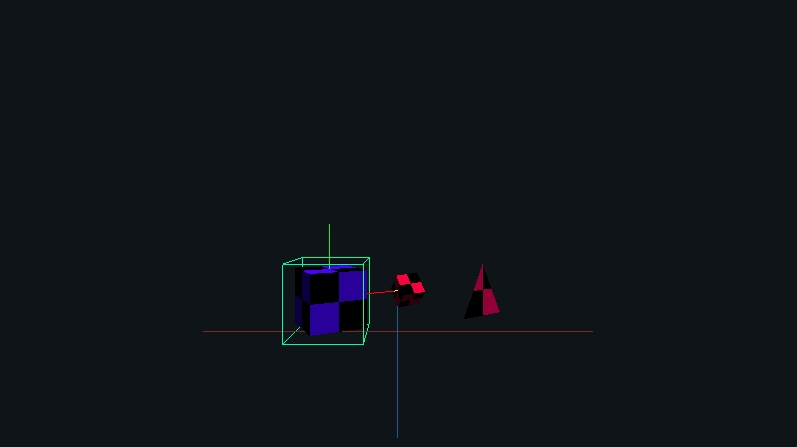
\includegraphics[width=0.9\linewidth]{images/showcase_scene.png}
\caption{Демонстрационная сцена \texttt{ShowcaseScene}}
\label{fig:showcase-scene}
\end{figure}

Системные тесты сцены \texttt{ShowcaseScene} приведены в таблице~\ref{tab:showcase-system-tests}.

\begingroup
\small
\renewcommand{\arraystretch}{1.12}
\begin{xltabular}{\textwidth}{|p{0.30\textwidth}|p{0.34\textwidth}|X|}
\caption{Системное тестирование сцены \texttt{ShowcaseScene}\label{tab:showcase-system-tests}}\\
\hline
\centrow Сценарий & \centrow Ожидаемый результат & \centrow Фактический результат \\
\hline
\endfirsthead
\caption*{Продолжение таблицы \ref{tab:showcase-system-tests}}\\
\hline
\centrow Сценарий & \centrow Ожидаемый результат & \centrow Фактический результат \\
\hline
\finishhead
Запуск класса \texttt{common.showcase.ShowcaseScene}. & Создается окно приложения, загружается сцена, отображаются трехмерные объекты. & Окно приложения создано, сцена загружена, на экране отображаются кубы, пол и отладочные направляющие. \\
\hline
Осмотр сцены свободной камерой. & При использовании клавиш перемещения и мыши камера меняет положение и направление обзора. & Камера перемещается по сцене и поворачивается вслед за движением мыши, обзор объектов меняется без перезапуска сцены. \\
\hline
Проверка иерархии трансформаций. & Дочерний куб движется относительно родительского объекта, сохраняя связь с ним. & Дочерний куб сохраняет положение относительно родительского объекта и изменяет мировое положение вместе с ним. \\
\hline
Проверка отладочной визуализации. & В сцене отображаются направляющие линии и вспомогательная геометрия, формируемая \texttt{DebugRenderer}. & Отладочные линии отображаются поверх основной сцены и обновляются при изменении положения объектов. \\
\hline
Проверка слоев и отсечения объектов. & Объекты, исключенные маской камеры или находящиеся за дальнюю плоскость отсечения, не отображаются в основной сцене. & Объекты с неподходящим слоем и объекты за пределами области видимости камеры не попадают в отображаемую часть сцены. \\
\hline
\end{xltabular}
\renewcommand{\arraystretch}{1.0}
\endgroup

\subsubsection{Проверка сцены \texttt{Interactive2DScene}}

Сцена \texttt{Interactive2DScene} предназначена для проверки ортографической
камеры, преобразования координат курсора в пространство сцены и работы
пользовательских скриптов интерактивных объектов. Место для скриншота сцены
приведено на рисунке~\ref{fig:interactive-2d-scene}.

\begin{figure}[H]
\centering
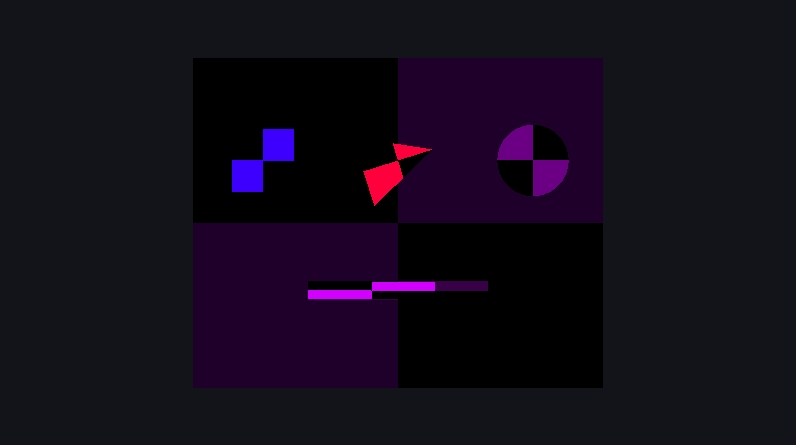
\includegraphics[width=0.9\linewidth]{images/interactive_2d_scene.png}
\caption{Демонстрационная сцена \texttt{Interactive2DScene}}
\label{fig:interactive-2d-scene}
\end{figure}

Системные тесты сцены \texttt{Interactive2DScene} приведены в
таблице~\ref{tab:interactive-system-tests}.

\begingroup
\small
\renewcommand{\arraystretch}{1.12}
\begin{xltabular}{\textwidth}{|p{0.30\textwidth}|p{0.34\textwidth}|X|}
\caption{Системное тестирование сцены \texttt{Interactive2DScene}\label{tab:interactive-system-tests}}\\
\hline
\centrow Сценарий & \centrow Ожидаемый результат & \centrow Фактический результат \\
\hline
\endfirsthead
\caption*{Продолжение таблицы \ref{tab:interactive-system-tests}}\\
\hline
\centrow Сценарий & \centrow Ожидаемый результат & \centrow Фактический результат \\
\hline
\finishhead
Запуск класса \texttt{common.showcase.Interactive2DScene}. & Создается окно приложения, отображается двумерная сцена с ортографической камерой и интерактивными объектами. & Окно создано, отображаются фон, кнопка, переключатель, слайдер и остальные объекты двумерной сцены. \\
\hline
Перемещение курсора над объектами сцены. & Скрипт отслеживания мыши корректно получает положение курсора в координатах сцены. & При перемещении курсора скрипт получает обновленные координаты в пространстве сцены, что используется для проверки наведения. \\
\hline
Нажатие на кнопку изменения цвета. & Визуальное состояние соответствующего объекта изменяется после клика мышью. & После клика объект меняет цвет, изменение сохраняется до следующего действия пользователя. \\
\hline
Нажатие на переключатель вращения. & Объект-переключатель изменяет режим поведения, вращение включается или отключается. & После нажатия переключатель меняет состояние, а связанный объект начинает вращаться или останавливается. \\
\hline
Взаимодействие со слайдером. & Заполненная часть слайдера меняет масштаб в зависимости от положения курсора и действия пользователя. & При перетаскивании указателя заполненная часть слайдера изменяет размер пропорционально положению курсора. \\
\hline
\end{xltabular}
\renewcommand{\arraystretch}{1.0}
\endgroup

\subsubsection{Проверка сцены \texttt{TexturedLightingScene}}

Сцена \texttt{TexturedLightingScene} предназначена для проверки материалов,
процедурно созданных текстур, передачи текстурных данных в OpenGL и работы
анимированного источника направленного света. Место для скриншота сцены
приведено на рисунке~\ref{fig:textured-lighting-scene}.

\begin{figure}[H]
\centering
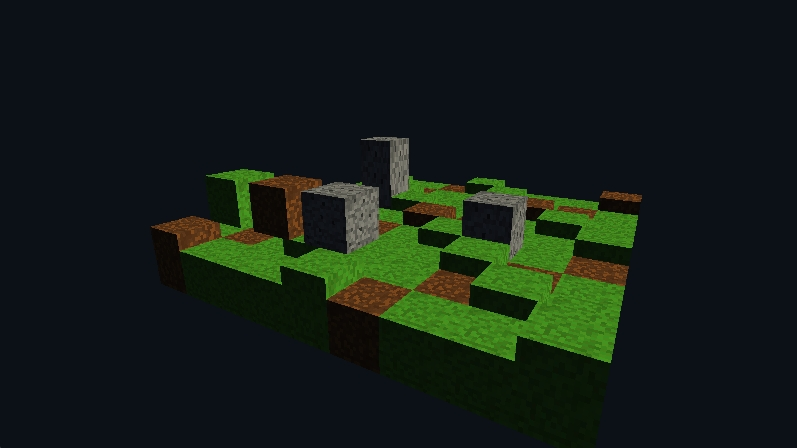
\includegraphics[width=0.9\linewidth]{images/textured_lighting_scene.png}
\caption{Демонстрационная сцена \texttt{TexturedLightingScene}}
\label{fig:textured-lighting-scene}
\end{figure}

Системные тесты сцены \texttt{TexturedLightingScene} приведены в
таблице~\ref{tab:textured-system-tests}.

\begingroup
\small
\renewcommand{\arraystretch}{1.12}
\begin{xltabular}{\textwidth}{|p{0.30\textwidth}|p{0.34\textwidth}|X|}
\caption{Системное тестирование сцены \texttt{TexturedLightingScene}\label{tab:textured-system-tests}}\\
\hline
\centrow Сценарий & \centrow Ожидаемый результат & \centrow Фактический результат \\
\hline
\endfirsthead
\caption*{Продолжение таблицы \ref{tab:textured-system-tests}}\\
\hline
\centrow Сценарий & \centrow Ожидаемый результат & \centrow Фактический результат \\
\hline
\finishhead
Запуск класса \texttt{common.showcase.}\newline
\texttt{TexturedLightingScene}. & Создается окно приложения, отображается сцена с несколькими текстурированными объектами. & Окно создано, сцена загружена, на объектах видны разные текстуры и освещенные грани. \\
\hline
Проверка процедурных текстур. & На объектах отображаются разные визуальные текстуры, созданные программно. & Объекты получают отличающиеся процедурные изображения, повторной загрузки файлов текстур не требуется. \\
\hline
Проверка направленного освещения. & Освещение влияет на видимые грани объектов, сцена не выглядит плоской. & Грани объектов имеют разную яркость в зависимости от направления света и нормалей поверхности. \\
\hline
Проверка анимации источника света. & Скрипт \texttt{OrbitingLightScript} изменяет параметры света во времени, что визуально влияет на освещение сцены. & В процессе работы сцены направление света изменяется, освещенные и затененные стороны объектов плавно меняются. \\
\hline
Проверка освобождения текстур. & При завершении сцены скрипт очистки и контекст приложения освобождают созданные ресурсы. & При закрытии сцены выполняется очистка процедурных текстур и связанных OpenGL-ресурсов без аварийного завершения. \\
\hline
\end{xltabular}
\renewcommand{\arraystretch}{1.0}
\endgroup

\subsubsection{Проверка сцены \texttt{PhysicsScene}}

Сцена \texttt{PhysicsScene} предназначена для комплексной проверки физической
подсистемы и ее взаимодействия с рендерингом, вводом, скриптами, камерой и
отладочной визуализацией. В сцене присутствуют динамические тела, статическое
окружение, узкая опора, кинематическая платформа, отладочная сетка и перезапуск
по клавише \texttt{R}.

Место для основного скриншота сцены приведено на рисунке~\ref{fig:physics-scene}.

\begin{figure}[H]
\centering
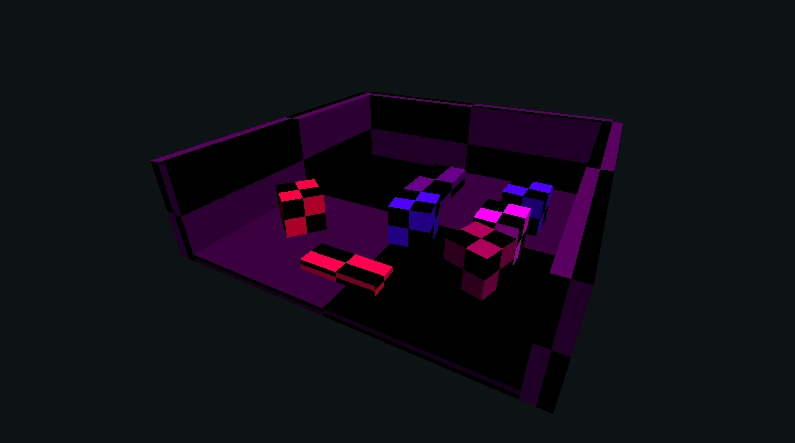
\includegraphics[width=0.9\linewidth]{images/physics_scene.png}
\caption{Демонстрационная сцена \texttt{PhysicsScene}}
\label{fig:physics-scene}
\end{figure}

Место для скриншота отладочной визуализации физической сцены приведено на
рисунке~\ref{fig:physics-debug-scene}.

\begin{figure}[H]
\centering
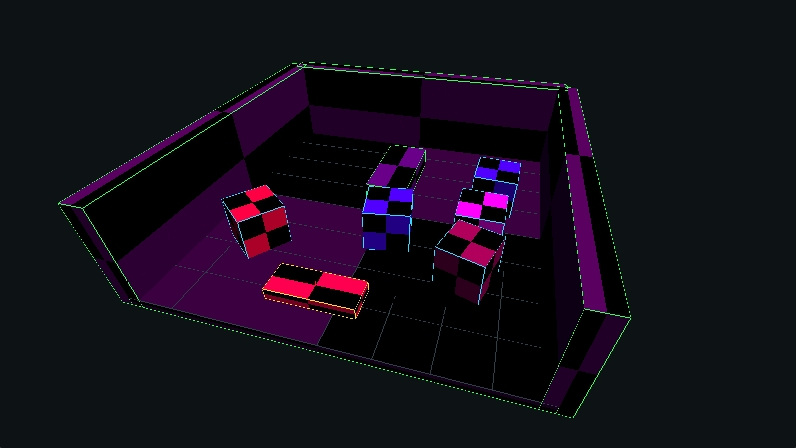
\includegraphics[width=0.9\linewidth]{images/physics_debug_scene.png}
\caption{Отладочная визуализация коллайдеров в сцене \texttt{PhysicsScene}}
\label{fig:physics-debug-scene}
\end{figure}

Системные тесты сцены \texttt{PhysicsScene} приведены в таблице~\ref{tab:physics-system-tests}.

\begingroup
\small
\renewcommand{\arraystretch}{1.12}
\begin{xltabular}{\textwidth}{|p{0.30\textwidth}|p{0.34\textwidth}|X|}
\caption{Системное тестирование сцены \texttt{PhysicsScene}\label{tab:physics-system-tests}}\\
\hline
\centrow Сценарий & \centrow Ожидаемый результат & \centrow Фактический результат \\
\hline
\endfirsthead
\caption*{Продолжение таблицы \ref{tab:physics-system-tests}}\\
\hline
\centrow Сценарий & \centrow Ожидаемый результат & \centrow Фактический результат \\
\hline
\finishhead
Запуск класса \texttt{common.showcase.PhysicsScene}. & Создается окно приложения, загружается физическая сцена, отображаются пол, стены, платформа и динамические кубы. & Окно приложения создано, физическая сцена загружена, видны статические объекты, платформа и набор динамических кубов. \\
\hline
Наблюдение за падением динамических кубов. & Кубы падают под действием гравитации и останавливаются на полу, опоре или платформе. & Динамические кубы перемещаются вниз, сталкиваются с опорными поверхностями и после затухания движения переходят в состояние покоя. \\
\hline
Проверка движущейся кинематической платформы. & Платформа перемещается между заданными границами, меняет направление и взаимодействует с динамическими объектами. & Платформа периодически меняет направление движения, а находящиеся рядом динамические объекты реагируют на контакт с ней. \\
\hline
Проверка столкновения со статическими объектами. & Динамические объекты сталкиваются с полом, стенами и узкой опорой, не проходят сквозь них и получают реалистичное изменение движения. & Кубы не проходят сквозь пол, стены и узкую опору; при смещенном контакте появляется падение или вращение. \\
\hline
Проверка отладочной сетки и визуализации коллайдеров. & В сцене отображается вспомогательная сетка и границы коллайдеров, позволяющие визуально сопоставить физические формы с графическими объектами. & Отладочная сетка и границы коллайдеров отображаются в сцене и визуально совпадают с положением физических объектов. \\
\hline
Перезапуск сцены по клавише \texttt{R}. & При нажатии клавиши выполняется запрос замены активной сцены, объекты возвращаются в исходные положения. & После нажатия клавиши \texttt{R} активная сцена заменяется новой, динамические объекты возвращаются в начальные положения. \\
\hline
\end{xltabular}
\renewcommand{\arraystretch}{1.0}
\endgroup
